\documentclass[10pt, a4paper, titlepage, draft]{report}
\usepackage{titlesec}% http://ctan.org/pkg/titlesec
\setcounter{secnumdepth}{5}
\titleformat{\section}%
	[hang]% <shape>
	{\normalfont\bfseries\Large}% <format>
	{}% <label>
	{0pt}% <sep>
	{}% <before code>
	
\titleformat{\subsection}%
	[hang]
    {\fontsize{13}{15}\normalfont\bfseries}
    {\thesubsection}
    {1em}
    {}
	
\titleformat{\subsubsection}
	[hang]
    {\fontsize{12}{14}\normalfont\bfseries}
    {\thesubsection}
    {1em}	
    {}
	
\titleformat{\paragraph}
	[hang]
	{\fontsize{10}{12}\normalfont\bfseries}
	{\theparagraph}
	{1em}
	{}
\usepackage[round]{natbib}
\usepackage{url}
\usepackage{breakurl} 
\usepackage[breaklinks]{hyperref}
\renewcommand{\baselinestretch}{1.5}
\begin{document}
\title{Automated HRTF Individualisation Based on Localization Errors in 3D Space}
\author{Robin Yonge}
\date{August 2017}
\maketitle


\section*{Background}
TODO:
sort out subsubsection topics to make it more elegant,
fill out notes'd bits,
maybe refer to this bit as introduction or motivation?

\subsubsection{How Humans Localise Sound/What do I mean by spatial audio?}
add in a bit about this, citing blauert, ez


\subsubsection{The Present Importance of Spatial Audio etc}
Spatial audio has never been more important. Though there has been a steady stream of interest in applications of spatial audio in fields like defence - primarily applied to Virtual Auditory Displays (VADs)\citep{•} - virtual, augmented, and mixed reality form a large component of the current technological zeitgeist. One major stated goal of these technologies is that of immersion. This doesn't have to mean that the user feels as if they have been transported to somewhere completely new, they just have to believe in the virtual elements of the experience. No matter whether the intended application is entertainment, productivity, or assistance (unsure about this line), the end user must be deceived into believing in what they are experiencing. 

Audio has parity with visuals here, as just small errors in either can irreparably break immersion\citep{•}.

[something about binaural audio here??? Explain meaning etc???
hrtfs as the principal determinant of sound localisation blah
Reproducing spatial audio convincingly involves a number of factors, including reflections and occlusion caused by the room and the objects in it. This project however, will focus entirely on the effect the anthropometry of the listener has on the audio signal - the attenuation of the sound caused by the various body parts that they sound waves come into contact with. 

\subsubsection{Recreating Spatial Audio/Representing this change?? idk}
In most applications involving spatial audio, representing this attenuation is done using Head-Related Transfer Functions, or HRTFs, derived from their time-domain counterparts Head-Related Impulse Responses, or HRIRs. HRIR measurements are taken by placing microphones in the ears of a participant (human or mannequin) and measuring the impulse response resulting when a tone is played from a loudspeaker \citep{who did this first?}. This measurement process should be repeated for as many positions/points of origin around the participant as possible in order to maximise coverage and provide the greatest amount of information when it comes to using the information to process audio. This process is incredibly labour-intensive, requires specialist equipment, and can take hours to perform. As a result, there are few organisations capable of performing these measurements, and generating a set of HRTFs for most people is impractical at best. [maybe a section on databases]There are a few organisations that have assembled databases of HRTFs, that involve measurements from a range of participants. The two main differences in these databases are the number of source positions, and the number of participants. 

\paragraph{Source Positions:}The number of source positions varies from database to database [in the case of CIPIC it is every L degrees from N to M, in the case of ARI, it is every Y degree from X to Z, etc]
[add diagrams!]

\paragraph{Subjects:}
These databases may contain anything from data from a single mannequin in the case of the MIT KEMAR set \citep{Gardner1994}, to the CIPIC database's 45 subjects \citep{Algazi2001}, up to the 110-subjects-and-growing ARI HRTF database \citep{AcousticsResearchInstitute}. 

\paragraph{•}
[table of databases by subjects and participants maybe?]

\subsubsection{The Problem}
Because of the aforementioned difficulty in measuring HRTFs, data from these databases is commonly used in attempts to implement spatial audio solutions. In the simplest implementations, the audio sample is convolved with the HRIR, producing audio that appears to come, convincingly or otherwise, from the position in 3D space that the HRIR was originally measured from. 

The problem with using this data in any spatial audio implementations that are to be used in applications for the consumption of a wide range of end users, is that HRTF data is incredibly specific to the person the measurements have been taken from. Just small differences in the anthropometry of the measured participant and the end user can compromise the efficacy of the HRTF used\citep{•}. However, when one tries instead to use a generalised HRTF - derived from the average of a set of measurements, or from a mannequin like the KEMAR\citep{kemar mannequin?} - the processed audio becomes too average and the same problems arise as using an HRTF from a single human. When using HRTFs that are not well matched to the user, front/back and elevation confusion is very common \citep{•}. 

Re-mention that VR/AR is popular, and that audio is integral to the progression of the technology!!!!.

It follows, then, that in a system that implements binaural audio, the audio for a user would be processed using a set of HRTFs could be used to recreate audio in such a manner that the user would be able to accurately localise the source of a sound. As we have already established, the traditional method of measuring HRTFs is impractical for the vast majority of users, which leaves us at something of an impasse. We need a method for producing individualised sets of HRTFs with minimal specialist equipment, an easy user experience that does not require expert knowledge, as small a time investment as possible. 



\section*{Literature Review}
\subsection{Modifying HRTFs/Overview}
This idea of generating individualised sets of HRTFs without having to perform the complex measurements that would usually be required has existed since the 1990s \citep{Kulkarni1995}. The ideal scenario for commonplace spatial audio involves every user having access to an HRTF set that works for them. If traditional methods of measurements are impractical, then alternatives are necessary.

\subsection{Methods}
Investigations into HRTF individualisation have been done using a range methodologies, some involving just simple selection tasks and others complex tuning - adjusting multiple parameters against listening tests. Often these methods hinge on a specific model that is used to decompose the HRTF into individual parameters that can be manipulated independently in order to achieve meaningful control over the customisation process. In some cases these models also seek to make clear the relationship between the features of the HRTF and the features of the user - the morphological properties of the measuree being the primary determinant of generated HRIR this seems a logical approach. In these next few sections I will cover the main of the approaches that have been investigated to date, as well as their efficacy and why they are or are not well suited to this project. We will see that there is a definite overlap between these methods, leading to the idea that perhaps in a more comprehensive but laborious model for HRTF individualisation, a combination of these techniques might be used \citep{Hoene2017}.

\subsubsection{Database Matching}
Database matching is often incorporated into other models for HRTF individualisation, and is somewhat self-explanatory. It is based on the predicate that within a database of a given size, there must be a set of HRTF measurements that have been taken from a participant with similar anthropometric features as a given user. This technique has been used in a range of studies on spatial audio, both as part of a wider study on binaural audio and localisation, \citep{Zotkin2002} and as the sole focus of the study \citep{Zotkin}. As in both of these papers from Zotkin et al, many attempts to match participants with closely matching HRTF sets use measurements of the user's anthropometry, which they will then try to match to the anthropometric measurements taken in the process of assembling the database. 

This can work reasonably well, assuming the database used contains measurements from a great enough range of people. The CIPIC database contains anthropometric measurements for all 45 of its participants \citep{•}, while the ARI database comes with measurements for 50 of its participants \citep{ARI site docs}. Problems  with this method can of course arise when the database does not include measurements from a participant with a morphology that does not closely match those of the user. The second problem with this method is more of an issue when considering this method in terms of what this project hopes to achieve. Given the my requirements for the customisation method I intend to design, a method that requires precise measurements that would be difficult to perform at home is not ideal. A method that requires precise measurements to be taken has two problems, both in the difficulty of performing the measurements, and the effort that such an act involves, does not satisfy any of my self-imposed standards for user experience.

An alternative method for matching users to their closest-matching HRTF set could be based on subjective listening tests. Playing a user a sample, filtered using an HRTF taken from a database, and asking them to indicate where they believed the sound came from. This process can be repeated for as many examples as are contained in the database, and the one that results in the least incorrect localisation attempts chosen. The problems with this method are again clear, in that the labour required to search all the entries in a database is more than anyone but the most die-hard users are likely to pursue [citation for some human-computer interaction junk about how much effort people will put in?]. Improvements are made on these kinds of subjective listening tests, however, in attempts to match users to more appropriate HRTFs through the clustering of similar sets. 

\subsubsection{Clustering}
Clustering involves collating a database of HRTF sets measured from different participants, and then sorting these into orthogonal groups based on a specific feature. Fahn and Lo in their 2003 paper \citep{Fahn2003} grouped HRTFs based on the power cepstra of each HRTF set. They then used a modified version of the LBG algorithm to form 6 different clusters. Other studies, such as a 2013 paper by Xie et al \cite{xie2013a} found a total of 7 clusters were required. Either way, the idea is to group HRTFs into groups - or clusters - where each HRTF is similar enough to the others in the cluster, but where the differences between each cluster are sufficiently great. You can then take the central example from each cluster, the HRTF that best represents that cluster or that represents the average, and provide to the end user the example from this set of 6 or 7 that best matches them. 

Given that clustering is meant to make simpler the process of matching a user with a more personal HRTF set, trying to match users by anthropometry again would be nonsensical. Instead, subjective listening tests are used more often \cite{xie2013a} \citep{•}. Using this method, the comparative efficacy of subejctive tests in this instance is clear versus raw database matching. As opposed to subjecting an undending barrage of tests against 45 or more (as a slightly facetious example), the listener has to compare between 6 or 7. However, the resulting localisation is going to be less precise, given the inherently more generalised approach. The increase in user-friendliness it interesting, though. In lighter-weight applications of VR/AR, perhaps for example on mobile devices, this approach could work. Giving interested users the option to choose between a subset of sufficiently disparate HRTFs, adding a little lightweight customisation. 

\citep{doi:10.1080/00140131003675117}
\citep{shimada1994a}

\subsubsection{Frequency Scaling}
Another methodology is based upon scaling in frequency entire HRTFs or elements of the HRTF. A method that was investigated early on in attempts to devise individualisation methods, it is one that lost out to cluster/database matching methods in the longer run. 

Some notable examples of studies into this technique include one by Middlebrooks \cite{Middlebrooks1999a}. In this study, they used Directional Transfer Functions (DTFs) which are processed HRTFs with the source location information isolated \cite{middlebrooks1990}. Initially finding that spectral features from one participant's DTF could be aligned with those of another by scaling. In further investigation participants used DTFs from the other participants, which were then scaled by a range of different factors based on comparisons in the two participants anthropometry - primarily the size of the head, and pinnae. This study then compared the participant's ability to localise sounds convolved with another's DTF against localisation when using the scaled DTFs and found a roughly 50\% increase in accuracy with the most effective scale factor. 

Another method investigated by Tan et al \cite{Tan1998}, involved building a tool that allowed users to manipulate the scaling of an HRTF themselves. Given that front/back and elevation confusion is most common when using non-individual HRTFs, they opted to provide options to add a bias towards the front/back, as well as another parameter to tweak how elevation was perceived. Their results showed an improvement over the non-individualised HRTFs, but not a substantial enough one. Given the simplicity of adjusting a mere two parameters this approach could have been very convenient. But the lack of an impressive improvement in localisation makes it a less tenable solution than some of the others explored, and it is overshadowed by later methods. 

\subsubsection{Structural Models}
Structural models appear to be the most commonly studied models for understanding HRTFs as well as for attempting to synthesise individual sets or customise generalised sets[I have roughly a billion citations for this, should I just plonk them all here?].  Because HRTFs and HRIRs represent the affects on the sound signal/wave of the features of a human's body, then one should be able to extract and isolate the discrete elements an HRTF that relate to the individual body parts. A German researcher by the name of Klaus Genuit first proposed a model for understanding HRTFs as a series of filters that each represented the effects of a certain anatomical feature \citep{Genuit1984}. The idea of a structural model, or of HRTF individualisation based on a user's anthropometry is pervasive, and many other methods incorporate elements from it. For example the aforementioned 2003 study by Zotkin, Duraiswami, Davis, and Hwang  \citep{Duraiswami2003} used anthropometric measurements to match a user to closely-matching set of HRTFs from the CIPIC database. Similarly, later studies centered on Principal Components Analysis - something I will go into in more detail later - look at the relationship between principal components (PCs) and morphological features. 

1998 work by Philip Brown and Richard Duda \cite{PhillipBrown1998} (itself based on a 1996 paper \cite{lopexmeddis1996}) looked primarily at HRIRs, focusing on the additional temporal information that the frequency-domain HRTFs lacked. The decision to focus on the time domain was to allow them to identify the characteristics of HRTFs that are the result of the different paths to the inner ear that the sound waves took, over time. This study involved only a small number of participants, and so whether or not the synthesised HRTFs produced with this model could replace measured ones is left to more comprehensive studies. 

In a 2001 study by 

\subsubsection{Principal Components Analysis}

\paragraph{Understanding PCA}

\paragraph{PCA and HRTFs/HRIR}
test citation \citep{Holzl2012a} 
\subsection{Search Methods}

\subsubsection{Simulated Annealing}

\section*{Method}
Based on the research outlined in the previous chapter, it was decided that an initial implementation of the proposed process would involve modelling the HRTF using principal components analysis to limit the number of variables in play to those those most significant components. Modifications to this reduced dataset would then be made based on simulated annealing search - with adjustments made where necessary. The efficacy of this implementation of this proposed approach has then been evaluated through listening tests conducted within a simple virtual reality environment. The metric for success is the same as the heuristic being used in the individualisation process - does the participant's ability to localise sound sources get better over time? If so, by how much?

\section{Algorithmic Design}
\subsection{PCA}
For this implementation I elected to follow the model for PCA and PCW weight adjustment outlined by Josef Holzl\citep{Holzl2014a}. The core implementation would largely follow his formulation, as mapped out in the paper, with modifications where necessary. This method allows for adaptation of the entire HRTF at once and helps to simplify the calculations that need to take place during the individualisation process, a convenience when a lot of the processing is taking place in real time. The input matrix structure that was decided upon during Holzl's investigation, [(Directions x Subjects)(Frequencies x 2)], was modified slightly to work for a single user to become: [Directions x (Frequencies x 2)]. In practical terms, an entry from the CIPIC HRIR database would be transformed into the frequency domain, resulting in an HRTF dataset in the form [Left/Right (2) x Azimuths (25) x Elevations (50) x Frequencies (101)]. This is then restructured into the above form, resulting in a structure [(Azimuths, Elevations (1250)) x (Frequencies, Left/Right (202))] in size. This structure is intuitive in terms of how the original values map to the new one, a quality that carries over even after the structure has been transformed with PCA. Performing PCA on this matrix effectively singles out the frequency bins that contain the most variance over all source directions. The resulting [PCW x PC] matrix is equivalent to [Directions x PCs] where the PCs are the frequency bins of greatest variance and the directions the PCWs. The benefit of this resulting structure is that it becomes very easy to modify the PCWs that relate to the position of a sound source. So for my implementation this means that it is simple to map the degree to which a user is able to locate a sound source to a relevant PCW within each PC. Because of this ability to match sound sources with principal component weights, coupled with the fact that PCW modifications were to be automated rather than performed manually, I chose not to model the resulting PCWs using spherical harmonics as Holzl did, further simplifying the individualisation process. 

The PCA model produced by this input matrix allows for around ninety percent of the variance in the to be described by 10 PCs, greatly limiting the number of variables that can be modified. This means that to adjust the perceived source of a sample the algorithm needs to only modify ten PCWs, one for each PCW that corresponds to that source position in each PC. 

\subsection{Simulated Annealing}
Core to simulated annealing (SA) search is that the degree of randomness, or the range of potential child states, is reduced as the current state gets closer to the goal state. In this implementation of the algorithm the value that is used to update the PCW is derived from user's localisation error, so the closer the user is to locating the sound source correctly, the smaller the change that is made to the PCW. It is worth noting that this implementation of this search method is effectively running 1250 individual searches in parallel, in order to find the optimal value for every individual source position so the process is unfortunately slow - this quality will be addressed in testing by limiting the number of possible source positions so that the effect of SA on individual source positions over time may be examined.

As mentioned above, modifying PCWs like this means that generating an individualised HRTF set would take at least 1250 seperate measurements, something that is almost as laborious as the standard measurement procedure. So to expedite the process, and to affect a greater amount of the HRTF with each modification, the PCWs for the eight source positions directly around the source being tested will also be modified by the same value, halved. This may mean that subsequent modifications partially overwrite previous ones, but it is preferable to expedite the process at least while data on the relationship between PCWs and localisation errors is so limited. This feature becomes somewhat irrelevant in the actual listening tests, but is of interest when considering the practical application of the algorithm.

Because there will be a not-insignificant amount of time betweeen each alteration made to a given PCW, the details of each alteration made are stored for future measurements from the same source position. This means that each time the algorithm begins to modify a set of PCWs, it first checks the database for previous adjustments. If extant, the previous error value, the modifier value for each PCW, and the change directions (whether the modifier was added to or subtracted from the weight within that PC) are all returned, and can inform this and subsequent changes. The direction of change is informed by whether or not this localisation attempt fared better than the previous one. If it did, then the change is made in the same direction. If it did not, some PCWs are adjusted the other way. In the event that a change is reversed and the next localisation attempt is better than the last, this system will ensure that the next change is made in the same direction(s). Given the aforementioned lack of research regarding the effect of the modification of different PCs on the perceived source of the sound, a decision had to be made regarding whether or not the update value was to be added to or subtracted from the current value of the PCW. The two options were to update every relevant PCW in the same direction, or to vary it. I decided on the latter, using different update directions in order to try and avoid situations where the algorithm might get caught in a loop, oscillating between two near-optimal states. The change was implemented using a process borrowed from genetic algorithms\citep{Whitley1994}, in which elements of a bit string are inverted based on a pseudorandom selection  process, coupled with the SA's decreasing degrees of randomness. In this implementation a number of indexes in the update-directions matrix are selected at random, but the exact number that are selected is determined again by the degree of error in the user's localisation attempt. This solution should result in steadily more granular changes as the HRTF set becomes more well-suited to the user. 

\section{Implementation}
The project that has been produced to test this proposed method is formed of three parts: A VR test environment that manages the positions of the sound sources and processes the audio samples, passing data to another module for processing. This individualisation module forms the core of the implementation, as it handles the deconstruction, modification, and reconstruction of the HRTF data. This module is then tied to an in-memory key-value datastore that holds the starting HRTFs, intermediate results, and an archive of the changes made so far. In this test implementation the VR environment and individualisation module run on different machines. This was necessary for ease of development, but it is also an interesting idea for potential future implementations using a similar method. If such a system could be built to aggregate PCW/localisation error data, using it to train a model that takes that data and returns customised HRTFs, it could benefit from the input of a larger amount of data than a method that ran exclusively locally. 

\begin{figure}
	\caption{HRTF Individualiser system diagram. }
	\centering{
		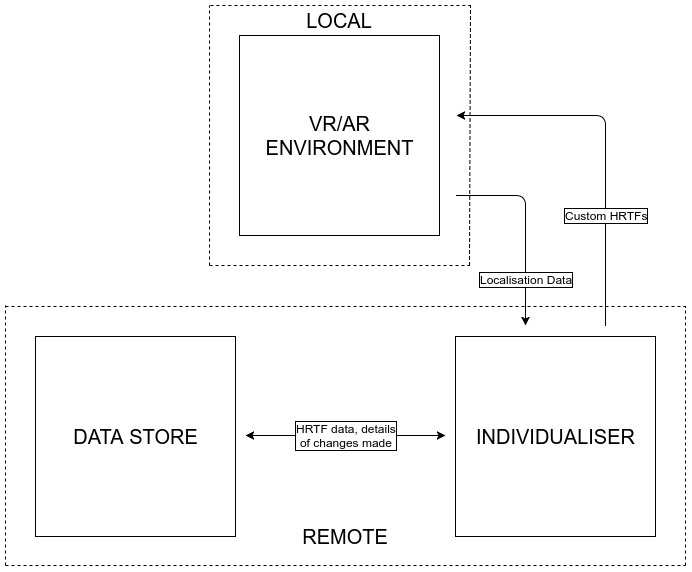
\includegraphics[scale=0.6]{individualiser_system_diagram}
	}
\end{figure}

\subsection{Technologies}
The bulk of the implementation is written in Python\citep{python lol}, making liberal use of the SciPy\citep{scipy and numpy} set of libraries to handle the majority of processing involved. Also in use is the simplejson\citep{simplejson} module, used to encode both HRTF data and logs extensively. To handle principal components analysis, the scikit-learn\citep{scikit learn} PCA class from the decomposition module was employed. Lastly, interfacing with the database was done using the lmdb module\citep{lmdb}. Symas' Lightning Memory-mapped Database \citep{lmdb db} was chosen both because it is a simple key-value datastore that doesn't require the kind of strictly defined strucure a relational database might, and because the entire contents of it can be loaded into memory when the program is started, making fetch and store operations comparatively rapid - useful when working in real-time. The test environment was produced using the Unity game engine \citep{•}, with the GoogleVR SDK \citep{•} and the Final Wireframe \citep{•} shader pack and run on a smartphone inside a Daydream\citep{•} viewer. Lastly, the individualiser module and production database are hosted on an Amazon Web Services (AWS) EC2 instance and communicate with the VR environment via TCP.

\subsection{Process}
Typically the individualisation process would run as follows, beginning with the user or participant in the VR space that is being used to generate the data. 

\begin{itemize}
\item The user faces a marker signifying the direction that relates to the 0, 0 angular coordinate for the CIPIC database.
\item The user is then played an audio cue that has been convolved with the corresponding HRIR from a source position that is generated at random but corresonds to a source position available in the database - in the case of the CIPIC database, this is anything from -45 degrees and up.
\item  Next, the user should point a reticle situated in the centre of their screen at where they think the sound originated from and issue some kind of confirmation. 
\item The perceived and actual sound source positions are then passed to the core module.
\item This information is then transformed into angular coordinates that match the way the CIPIC data is arranged, from which the update value is calculated like so:
\begin{itemize}
\item The perceived source position is subtracted from the actual source position, and divided by ten. 
\item These two values are each multiplied by a weight value, which was set to 0.6 during the listening tests, and summed together. 
\end{itemize}
This process is somewhat arbitrary, and mostly serves to generate a value between zero and three. This threshold is based on Holzl's implementation, and introduction of the weight value into the calculation process is primarily to allow easier adjustment prior to testing. 
\item The current individualisation-in-progress HRTF is then fetched from the database, along with a pre-prepared PCA model, and reformed into a [1250 x 202] input matrix. 
\item Next a matrix containing the mean value of each column in this matrix is subtracted from the input matrix and stored for later. 
\item The input matrix minus the mean is transformed using the PCA model, to produce the [1250 x 10] [PCWs x PCs] matrix. 
\item The database is then queried, to see if a modification has been made to this source position before, and the update value is used to adjust the PCWs according to the following conditions:
\begin{itemize}
\item If there is no data about previous adjustments, a set of ten boolean values are generated using Python's random module\citep{python random} to represent the adjustment direction for each principal component for that this weight (source position). 
\item Otherwise, if the data exists and the difference between the perceived and actual source positions in the most recent localisation attempt is greater than the previous one, a randomly chosen subset of the previously-used set of booleans have their values reversed and each PC is adjusted according to those directions. Otherwise, if the difference is lower, make the adjustment in the same direction. 
\end{itemize}
\item Information on the details of the adjustment made are then stored in the database, overwriting any previous data for changes made to that direction.
\item Once the PC matrix has been updated, the PCA transform is performed in reverse, and the column mean values are added back in.
\item Finally, this matrix is re-structured into the same format as the original HRTF matrix and stored in the database under the same key it was fetched from, archiving the previous iteration. 
\item This new, modified, HRTF is then used to process the next audio sample played to the user, and the process begins again. 
\end{itemize}

\subsection{Testing}
When it comes to analysing the efficacy of the approach, the tests will largely follow the above process with some small deviations. Because of the limited time available with each participant, I have run the process with the random source positions limited to a smaller subset of 8 key directions as opposed to the 1250 possible source positions if working with the full dataset. Limiting the source positions like this has allowed me to ensure that over the course of each test we are able to iterate over each source position several times, getting a better idea of how the PCWs change over time in relation to the error rate, and how localisation accuracy might change for a given direction over time. This limited set of source positions will be located in front of, behind, and to the left and right of the participant, as well as on the eight corners making up a cube around the participant.

The position of the sound source will change pseudorandomly, ensuring that the subject is tested from each source position the same number of times and that the same position isn't used twice in a row. For each position, the participant will be asked to face forward while the test sample, a one-second clip of pink noise, processed with the (semi)customised hrtf. The participants will have the option to play the sample again if they wish, and will be given ample time to try to locate the source position as accurately as they can. There will also be an on-screen indicator that displays when the participant is facing forward, allowing them to monitor their own head position.

During the tests, the individualisation module will automatically capture and all necessary for analysis. This includes the source location, perceived location, and resulting error value, as well as all of the primary PCWs both before and after they have been updated and what the direction of each update. All of this data is also timestamped, to make it easier to group data both chronologically, and by test/participant. 

The main metric that I have analysed based on the tests is the error rate over time. In particular, whether or not there is any decline in error rates as the test progresses. As a secondary point of interest, I have tried to investigate whether or not any relationship between localisation errors, individual principal components, and update directions can be identified in my data. Any potential relationship that exists there is of note, because that information could be used to substantially enhance any future implementations of/updates to this individualisation process.

\section*{Analysis}
I was thinking I'd do a section for each metric/relationship I'm able to analyse

\section{Localisation Error Over Time}
start with description of the data being displayed on the charts and how the charts were generated (how data was processed and the technologies used)

\bigskip

Here I was thinking a graph or set of line charts displaying mean error rate for all participants over time for each source position, but twelve lines on a single chart might be too much? Unless it's one very large chart. So I was expecting to split it into three, one for each elevation - sources below the listener, sources at the same level, and sources above. There will also be only about 5 points along the X axis so they might all fit in a single line. Is there a well-defined style? Or should I just try both and go with whatever I think looks nicer?

\bigskip 

Then describe what the conclusions can be drawn from the data being displayed

\section{Relationships Between PCs and Localisation Errors}
Again, starting with a description of how the data was was collated from the tests, and how it was arranged on the charts. I just can't yet work out the best way of displaying the data for this. It would be nice to represent it on a sphere or section of a sphere, something like that? 

\bigskip

same structure, charts in between 

\bigskip 

Conclusions we can draw, etc

\section{•}
Then this structure could be repeated as needed, for as much analysis as I get to do??

\section*{Discussion}
Introducing this project, I defined my goal as being to produce a process with which to generate a individualised HRTF set based on user-generated data, without any more equipment or expertise than the average end user of a virtual, augmented, or mixed reality system might have, on a practical time scale. The process as it currently stands does not effectively meet these requirements, though I am confident that it is a good starting point - serving its function as a proof-of-concept. From a user experience standpoint, basing the individualisation process on the user's error in localisation is an approach which has the potential to be effective. There is sizable scope for gamification of the process using this method, which has the potential to encourage non-enthusiast users to undergo the process as these technologies become more widespread and their application areas become more diverse. To make it practical, however, the underlying algorithm would need to produce an individualised HRTF using a smaller amount of direct input from the user than is currently required. Using the current implementation, even if the rate of measurements were to be increased tenfold it would still take an untenably long time to produce an entire HRTF set, losing a potential point in favour of this type of method over the traditional measurement process. 

This leads into the greatest current problem with the produced implementation; it is unknown whether or not it would actually produce an effective custom HRTF set. This is part of the problem of choosing to base this project on SA, as I have discussed in previous chapters. Making pseudorandom changes to the HRTF data means that sub-optimal child states are regularly explored, and this slows the process down significantly. Given that my listening tests were limited to exploring six steps into the search process, it is difficult to estimate how many steps through the search would be required to reach a point at which the HRTF could be said to be fit the individual. Knowing, however, that it is greater than six means that it can be conluded that individualisation of a full set of HRTFs using this exact implementation is untenable.

\section{Improvements}

It is possible that some small modifications could make this method more effective, starting with the effects on perception that result from a given adjustment value. The current implementation was based on Josef Holzl's implementation\citep{Holzl2014}, that allowed adding or subtracting values up to three from the PCWs, but a more concerted look into the effects of different ways of calculating the adjustment value could be beneficial. It would also be worth reviewing the effect that different starting HRTF sets have on the process. As has been mentioned previously, it's impossible to find HRTF data that works for everyone. But it might be possible to find a small set that work broadly as starting points for individualisation. The starting HRTF could even be selected automatically based on a similar style of localisation test. 

It has already been covered heavily in previous chapters, but a better understanding of the relationship between the PCW adjustments being made and the effect that the adjustments will have on perception could be the greatest improvement while keeping the broader implementation details largely the same. We saw in the previous chapter that there appears to be some correlation between PCW adjustment and perceived source position, and with more focused research in this area it's possible that a much clearer relationship could be identified. Coupled with a better understanding of the change produced by a given adjustment value, this could help eliminate the early missteps in the search process and allow the algorithm to make more targeted adjustments sooner, greatly lowering the total number of steps required for individualisation.

Working from the assumption that enough data can be gathered, potentially through use of or research into a greatly improved version of the current algorithm, I think there is also scope to investigate the application of more complex machine learning algorithms to this process. There are plenty of obstacles ahead of making this feasible, but assuming they could all be overcome with sufficient research time then the ideal implementation might function as follows: As with the current implementation, it should start with a neutral/default HRTF, play the user a set of sounds from a predetermined set of positions, and ask them to locate where they believe they originated from. This data should be enough (the exact amount of data quantified with the design of the system) to feed into a pre-trained machine learning model that should then return a more individualised HRTF. Training such a model would take more data than appears to be currently available, and the time required to generate that data could be substantial. Though if there was the potential to build the ability to capture that data into a simpler system that was actively used, it could eventually be feasible. Such a system, fantastical though it may currently be, would fulfil all of the requirements that I initially defined, while hopefully offering improved an improved spatial audio experience for a wider range of people.


\bibliography{bibliography/library}
\bibliographystyle{plainnat}
\end{document}